\documentclass[10pt,fleqn]{article}

\usepackage[english]{babel}
\usepackage[utf8x]{inputenc}
\usepackage{enumerate}
\usepackage{amsmath}
\usepackage{amssymb}
\usepackage{amsfonts} 
\usepackage{mathtools}
\usepackage{graphicx}
\usepackage{bm}
\usepackage[usenames,dvipsnames]{color}
\usepackage{todonotes}
\usepackage{dsfont}
\usepackage{hyperref}
\hypersetup{
    colorlinks,
    citecolor=black,
    filecolor=black,
    linkcolor=black,
    urlcolor=black
}
\usepackage{algorithm}
\usepackage{algorithmic}
\usepackage{appendix}
\usepackage{subcaption}
\usepackage{fancyvrb}
\usepackage{subfigure}
\usepackage{graphicx,xcolor}
\usepackage{pifont,mdframed}
\usepackage{tikz}
\usepackage{bm}
\usetikzlibrary{fit,positioning}


%
% Macros
%
\newcommand \cashort[1] { {\todo[color=yello]{#1 -- Cedric}} }
\newcommand \calong[1]  { { \todo[inline,color=yellow]{#1 -- Cedric} } }
\newcommand \gbshort[1] { {\todo[color=cyan!40]{#1 -- Guillaume}} }
\newcommand \gblong[1]  { { \todo[inline, color=cyan!40]{#1 -- Guillaume} } }
\newcommand \mgshort[1] { {\todo{#1 -- Mark}} }
\newcommand \mglong[1]  { { \todo[inline]{#1 -- Mark} } }
\newcommand \bfshort[1] { {\todo[color=green!40]{#1 -- Bryan}} }
\newcommand \bflong[1]  { { \todo[inline,color=green!40]{#1 -- Bryan} } }


% Adds a plus const to the end of a math expression
\def \pcst{+\text{const}}

% A fancy version for capital R
\def \Rcal{\mathcal{R}}

% A fancy version for r
\def \rcal{\mathbf{r}}

% Loss function / log likelihood as appropriate
\def \L{\mathcal{L}}

% KL divergence [Math Mode]
\newcommand{\kl}[2] {
	\text{KL}\left[#1||#2\right]
}

\newcommand \vecf[1] {
    \text{vec}\left(#1\right)
}

\newcommand \ent[1] {
    \text{H} \left[ #1 \right]
}

\newcommand \mut[2] {
    \text{I} \left[ #1 ; #2 \right]
}

\newcommand \dvi[2] {
    \text{D}_\text{VI} \left[ #1; #2 \right]
}

% Starts an expected value expresses [Math Mode]
\newcommand{\starte}[1] {%
	\mathbb{E}_{#1}\left[
}

% Ends an expected value expression [Math Mode]
\def \ende{\right]}

% Starts an varianc expresses [Math Mode]
\newcommand{\startv}[1] {%
	\mathbb{V}\text{ar}_{#1}\left[
}

% Ends an variance expression [Math Mode]
\def \endv{\right]}

%\newcommand \ex[2] {
%    \bigl\langle #1 \bigr\rangle_{#2}
%}
\newcommand \ex[2] {
    \mathbb{E}_{ { #2 } }\left[ #1 \right]
}
\newcommand \var[2] {
    \mathbb{V}ar_{ { #2 } }\left[ #1 \right]
}

\newcommand \halve[1] {
	\frac{#1}{2}
}

\newcommand \half {
    \halve{1}
}

\newcommand \tr { \text{tr} } 

\newcommand \T { ^\top } 

\newcommand \fixme[1] {
    {\color{red} FIXME: #1}
}

\newcommand \vv[1] { \bm #1 }

\newcommand{\mbeq}{\overset{!}{=}}

\newcommand \diag[1] { \text{diag} \left( {#1} \right) }
\newcommand \diagonal[1] { \text{diagonal} \left( {#1} \right) }

\newcommand \Ed {{ \vv{\xi}_d}}
\newcommand \Edj {{\xi_{dj}}}
\newcommand \Edk {{\xi_{dk}}}
\newcommand \AEdj {{\Lambda(\xi_{dj})}}
\newcommand \AEdk {{\Lambda(\xi_{dk})}}
\newcommand \AEd  {{ \bm{\Lambda}(\bm{\xi}_d) }}

\newcommand \Axi { { \Lambda_{\xi} } }
\newcommand \bxi { { \vv{b}_{\xi} } }
\newcommand \cxi { { c_{\xi} } }


\newcommand \wdoc      { { \vv{w}_d } }
\newcommand \wdt[0]  { { w_{dt} } }
\newcommand \wdn[0]  { { \vv{w}_{dn} } }
\newcommand \wdnt[0]  { { w_{dnt} } }
\newcommand \wdd[0]   { { \vv w_{d} } }
\newcommand \zd[0]   { { \vv z_{d} } }
\newcommand \zdn[0]  { { \vv{z}_{dn} } }
\newcommand \zdnk[0] { { z_{dnk} } }
\newcommand \zdk[0]  { { z_{dk} } }
\newcommand \thd[0]  { { \vv \theta_d } }
\newcommand \thdk[0] { { \theta_{dk} } }
\newcommand \thdj[0] { { \theta_{dj} } }
\newcommand \epow[1] { { e^{#1} } }
\newcommand \pkt     { { \phi_{kt}  } }
\newcommand \pk      { { \vv \phi_k } }
\newcommand \lmd     { { \vv \lambda_d } }
\newcommand \lmdk    { { \lambda_{dk} } }
\newcommand \xd      { { \vv x_d } }
\newcommand \atxd     { A ^\top \bm x_d}
\newcommand \axd     { A\bm x_d}
\newcommand \tsq      { { \tau^2 } }
\newcommand \ssq      { { \sigma^2 } }
\newcommand \tmsq     { { \tau^{-2} } }
\newcommand \asq      { { \alpha^2 } }
\newcommand \amsq     { { \alpha^{-2} } }
\newcommand \sgsq     { { \sigma^2 } }
\newcommand \xvec     { { \vv{x} } }
\newcommand \omk      { { \bm \omega _k } }
\newcommand \omkt     { { \omega_{kt} } }
\newcommand \oma     { { \Omega_A } }
\newcommand \gdn      { { \vv{\gamma}_{dn} } }
\newcommand \gdnk     { { \gamma_{dnk} } }
\newcommand \gdk      { { \gamma_{dk} } }
\newcommand \isigt   { { \Sigma^{-1}_{\bm \theta} } }




\newcommand \halfSig { \frac{1}{2\sigma^2} }

\newcommand \nor[2]   { \mathcal{N} \left( {#1}, {#2} \right) }
\newcommand \nord[3]   { \mathcal{N}_{#1} \left( {#2}, {#3} \right) }
\newcommand \mnor[3]  { \mathcal{N} \left(#1, #2, #3\right) }
\newcommand \norp[3]  { \mathcal{N} \left(#1; #2, #3\right) }
\newcommand \mnorp[4] { \mathcal{N} \left(#1; #2, #3, #4\right) }
\newcommand \mul[1]   { \mathcal{M} \left( {#1} \right) }
\newcommand \muln[2]  { \mathcal{M} \left( {#1},{#2} \right) }
\newcommand \dir[1]   { \mathcal{D} \left( {#1} \right) }
\newcommand \pois[1]  { \mathcal{P} \left( {#1} \right) }
\newcommand \gp[2]    { \mathcal{GP} \left( {#1}, #2 \right) }
\newcommand \dir[1]   { \mathcal{D} \left( {#1} \right) }
\newcommand \gam[2]   { \mathcal{G} \left( {#1}, {#2} \right) }
\newcommand \beta[1]  { \mathcal{B}eta \left( {#1}, {#2} \right) }

\newcommand \lne[1]  { { \ln \left( 1 + e^{ #1 } \right) } }
\newcommand \Tr[1]   { \tr \left(  {#1}  \right) }

\newcommand \roud  { \vv{\rho}_{d}  }
\newcommand \rodk { \rho_{dk} }

\newcommand \exA[1]  { \ex{#1}{q(A)} }
\newcommand \exV[1]  { \ex{#1}{q(V)} }
\newcommand \exT[1]  { \ex{#1}{q(\Theta)} }
\newcommand \extd[1] { \ex{#1}{q(\thd)} }
\newcommand \exTV[1] { \ex{#1}{q(\Theta)q(V)} }

\newcommand \Real[0]  { { \mathbb{R} } }
\newcommand \VReal[1] { { \mathbb{R}^{#1} } }
\newcommand \MReal[2] { { \mathbb{R}^{#1 \times #2} } }
\newcommand \Nat[0]  { { \mathbb{N} } }
\newcommand \VNat[1] { { \mathbb{N}^{#1} } }
\newcommand \MNat[2] { { \mathbb{N}^{#1 \times #2} } }

\newcommand \inv[1] { {#1}^{-1} }
\newcommand \invb[1] { \inv{\left( #1 \right)} }

\newcommand \cn { \textsuperscript{\texttt{[{\color{blue}Citation Needed}]}} }

\newcommand \const { { \text{c} } }

\providecommand \floor [1] { \left \lfloor #1 \right \rfloor }
\providecommand \ceil [1] { \left \lceil #1 \right \rceil }


\newcommand \vt[2] { { #1^{(#2)} } }

\newcommand \hashtag[1] { { \ttfamily \##1 } }

\newcommand \mvy  { \vv{m}_{\vv{y}} }
\newcommand \sigvy { { S_Y } }

\newcommand \mmy  { M_Y      }
\newcommand \md   { \vv{m}_d }
\newcommand \phin { \vv{\phi}_n }
\newcommand \isigma { { \inv{\Sigma} } }

\newcommand \sigv     { { \Sigma_V } }
\newcommand \isigv     { { \Sigma^{-1}_V } }

\newcommand \sigy { { \Sigma_Y } }
\newcommand \isigy { { \Sigma_{-1}_Y } }


\newcommand \omy  { { \Omega_Y } }
\newcommand \iomy { { \inv{\Omega_Y} } }

\newcommand \siga     { { \Sigma_A } }
\newcommand \isiga     { { \Sigma^{-1}_A } }
\newcommand \diagv { { \diag{\nu_1,\ldots,\nu_P} } }

\newcommand \ma { \vv{m}_a }
\newcommand \my { \vv{m}_y }

\newcommand \VoU { V \otimes U }

\newcommand \one { \mathbb{1} }
%\newcommand \one  {{  \mathds{1} }}

\newcommand \lse { \text{lse} }
%\newcommand \lse[0] { \mathrm{lse} }

% Conditional independence 
\def\ci{\perp\!\!\!\perp} % from Wikipedia



% ------ For the eval section

% Multinomial PDF [Math Mode]
% params: 1 - the variable
%         2 - the value
%         3 - the state indicator (e.g. k for a distro with K values)
%         4 - any additional subscript
\newcommand{\mpdf}[4] {
	\prod_{#3} {#1}_{{#4} {#3}} ^ {#2}
}

% Dirichlet PDF [Math Mode]
% params: 1 - the variable
%         2 - the hyper-parameter
%         3 - the state indicator (e.g. k for a distro with K values)
%         4 - any additional subscript
\newcommand{\dpdf}[4] {
	\frac{1}{B({#2})} \prod_{#3} {#1}_{{#4} {#3}} ^ {({#2}_{#3} - 1)}
}

% To simplify the sampling equations, this is indicates
% that the given value has had datapoint "m" stripped out
%
\newcommand{\lm}[1] {
	#1^{\setminus m}
}

\newcommand \model[0] {
    \mathcal{M}
}

\newcommand \perplexity[1] {
    \mathcal{P} \left( { #1 } \right)
}

\newcommand \WTrain {
    \mathcal{W}^{(t)}
}

\newcommand \WQuery {
    \mathcal{W}^{(q)}
}

\newcommand \oneover[1] {
    \frac{1}{ {#1} }
}

\newcommand \samp[1] {
    { #1 }^{(s)}
}

\newcommand \etd[0] {
    \vv{\eta}_d
}

\begin{document}



\newcommand \thdo { { \vv{\theta}_{d\cdot} } }
\newcommand \thok { { \vv{\theta}_{\cdot k} } }
\newcommand \phok { { \vv{\phi}_{\cdot k} } }
\newcommand \phdo { { \vv{\phi}_{d\cdot} } }

\title{Self-Referential Matrix-Variate Topic Models for Citation Prediction}
\author{Bryan Feeney}
\maketitle
\section{Introduction}
As document corpora have grown ever larger, the need for improved methods to search within these corpora has grown. The simplest approach is to learn a low-rank representation of each document, for example using latent Dirichlet allocation (LDA)\cite{BleiNgJordan2003} to infer a distribution over the topics that best explain the contents of each document. 

In the case of document networks however, one also needs to incorporate network structure as well as words to explain the corpus. In particular, by modelling network structure, models can propose additional links, providing the basis for a recommendation engine. 

Most approaches to date have focussed on modelling the network as an unweighted graph (i.e. a link exists or does not), and frequently as an undirected graph. Oftentimes topic-modelling has been used as a separate feature extraction step, or has been incorporated into the model. The most successful discriminative approach has been the SVM approach of\cite{Bethard2010}, which classified documents as links or non-links according to features. They found the most influential features when predicting links were, in order: whether the link is a self-citation; a transitive self-citation with one step; the number of times the linked paper has been cited a priori; the words of the paper; it's age relative to the link origina; whether the cited and out-link papers shared a venue; and finally functions of the topics inferred from the words using LDA\cite{Blei2003}.

However learning topics in conjunction with, instead of separate from, the prediction problem, adds the advantage that the link structure can be used to help learn the topics. The typical approach is to learn topics from the text of a document, which simultaneously training a logistic regression model to predict whether a link should exist between two documents based on a function of their topics. Two possible features are available, the parameter of the Dirichlet posterior over topics for document $d$ $\thd$ or the average of per-word topic-assignments for document $\bar{\vv{z}}_d = \frac{1}{N_d} \sum_d \vv{z}_{dn}$.

Typically however, the topic distribution explain a document's words differs slightly from those predicting the origins of its inbound links, necessitating some adaptation. In the Relational Topic Model (RTM)\cite{Chang2009a}\cite{Chang2010a} the probability of a link from $d$ and $p$ is $p(y_{dp} = 1) = \sigma\left(\vv{\eta}\T(\bar{\vv{z}}_d .* \bar{\vv{z}}_p) + \nu \right)$ where $.*$ indicates the Hadamard product, the vector $\vv{eta}$ weights the distance and the scalar $\nu$ is some learnt random noise. By comparison, in \cite{Neiswanger2014} a separate noise term is learnt for each document when it is the target of a link, leading to the distribution $y_{dp} \sim \nor{\gamma \thd\T\vv{\theta}_p + \gamma \thd\T\vv{\epsilon}_p}{\tau_{y_{dp}}}$ where $\gamma$ scales the result to approximately $0\ldots 1$, and $\vv{\epsilon}_p$ is drawn from a Gaussian. Two different values of the variance $\tau$ are learnt depending on whether $y_{dp} = 1$ or $y_{dp} = 0$. 

The LDA/PLSA model\cite{Nallapati2008}\cite{Nallapati2008a} takes a slightly different approach. It starts with a multi-field topic-model approach\cite{Blei2003} where using a single Dirichlet prior over the $K$ topics parameterised by $\thd$, two sets of topic-assignments are drawn, one for words, and one for links. In the case of words, there are $K$ associated distributions over topic words. In the case of documents there are likewise $K$ distributions over topic documents. However to encourage this latter distribution to take into account document contents, both it and the per-topic vocabularies are simultaneously used to train a PLSA model. This requires learning two sets of topic assignments to model words (one for LDA and one for PLSA) in addition to the set of topics modelling links.

The SVM model of \cite{Bethard2010} is one of the few to consider time. In a generative setting \cite{Gerrish2010} modelled words only using an extension of thedynamic topic model of \cite{Blei2006a} in which time was quantized, and per-topic vocabularies changed between quanta according to a Kalman Filter style algorithm operating on the logistic-normal vocabulary distributions. The novel aspect of \cite{Gerrish2010} is in the addition of an impact factor, one for each paper and topic, which up-weights the contribution of that paper's topic-words when inferring the prior over vocabularies in the next time-step.

Link prediction is an unbalanced prediction problem, with very few positive examples in the dataset. In the case of \cite{Bethard2010} a variant of SVM optimising the MAP criterion\cite{Yue2007} (i.e. ranking) was found to outperform logistic regression and logistic regression with downsampled negative inputs. In the RTM model\cite{Chang2009a}\cite{Chang2010a} a single-class classifier was trained, regularised by using a combination of Gaussian priors and the addition of a number of pseudo-documents for the negative case drawn from the posterior, their number indicated by means of a parameter $\rho$. This was motivated by the fact that the absence of links cannot be construed as evidence indicating links should not exist, and therefore one should not employ the ``zeroes" in the dataset as negative samples when training a classifier. Other approaches have simply ignored the imbalance, or in the case of the Link-PSLA-LDA model\cite{Nallapati2008}\cite{Nallapati2008a} used a multinomial distribution over documents' out-links, whose posterior is a function solely of existing links (the ``ones").

An alternative approach is to use a form of weighted stochastic gradient descent, which preferably samples from the positive links rather than negative ones, while maintaining convergence guarantees. This was used in \cite{Gopalan2013b}\cite{Gopalan2013} though in network models which ignored document contents.

In this paper we propose a new model for link-prediction. Unlike the approaches discussed this far, we consider both the directionality and the \emph{weight} of links: for each document, we consider the number of times a paper has been cited. As in the Link-PSLA-LDA model we try to use the topics learnt from words of a document to model whether a document should be the recipient of a link. However we take a wholly Bayesian approach to this problem, using suitably configured priors to account for the fact that the topics which explain a documents words and "out-links" do not exactly model the "in-links" it receives as it is cited by subsequent work.

\section{The Matrix-Variate Normal Distribution}
Given a random matrix $X \in \MReal{D}{K} \sim \mnor{M}{\Sigma}{\Omega}$ with row covariance $\Sigma \in \MReal{K}{K}$ and column covariance $\Omega \in \MReal{D}{D}$ its log-pdf is given by
\begin{align}
\halve{DK}\ln 2\pi - \halve{D}\ln|\Sigma| - \halve{K} \ln|\Omega| -\Tr{\inv{\Omega}(X - M)\inv{\Sigma}(X - M)\T}
\end{align}
This is mathematically identical to the following distribution over the vectorized matrix X, $\vecf{X} \sim \nor{\vecf{M}}{\Omega \otimes \Sigma}$. It should be noticed that this approach, due to the assumed separability of the covariance, is a considerably more parsimonious model than naively assuming $\vecf{X} \sim \nor{\vecf{M}}{S}$. The separability assumption, i.e. that $S = \Omega \otimes \Sigma$ means that the covariance is approximated in the following ways:

\begin{align}
\cov{X_{dk}, X_{pj}} & = \Omega_{dp} \Sigma_{kj} &
\cov{X_{d-}} & = \Omega_{dd} \Sigma &
\cov{X_{-k}} & = \Sigma_{kk} \Omega \label{eqn:sep-cov-forms}
\end{align}


\section{The Model}
Following the example of the correlated topic model (CTM)\cite{Blei2006} we try to capture correlations between topics. We collect the individual document topic-score vectors $\thdo$ into a matrix $\Theta \in \MReal{D}{K}$. 
\begin{align}
\Theta &\sim \mnor{\vv{\mu}\one\T}{\Sigma}{\alpha I_D}
\end{align}

Denoting the softmax function as $\sigma_k(\vv{\theta}) = \frac{\theta_k}{\sum_j \theta_j}$ and the vector of softmax scores as $\vv{\sigma}(\vv{\theta})$ we 
the topic for the $n$-th of the $N^w_d$ words in document $d$ as
\begin{align}
\zdn & \sim \muln{\vv{\sigma}(\thdo)}{1} &
\wdn & \sim \muln{\vv{\lambda}_{z_{dn}}}{1}
\end{align}
And likewise for the $m$-th of the $N^l_d$ out-links in document $d$
\begin{align}
y_{dm} & \sim \muln{\vv{\sigma}(\thdo)}{1} &
l_{dp} & \sim \muln{\vv{\beta}_{- z_{dn}}}{1}
\end{align}

Were we to put simple Dirichlet priors over $\vv{\beta}_k$ and $\vv{\phi}_k$ we would just have a simple multi-fieldtopic-model\cite{Blei2003}. However we instead wish to transfer our knowledge of how topics are emitted by document $\Theta$ to the parameter $\Phi = \{ \vv{\phi}_k\T \}_{k=1}^K$ governing how documents are emitted for each topic $k$. Thus we use the following prior:
\begin{align}
\Phi|\Theta & \sim \mnor{\Theta}{\Sigma}{\diag{\vv{\rho}}}
\end{align}
where $\vv{\rho} \in \VReal{D}$ is the column covariance of all documents, and takes into account our uncertainty with regard to individual documents' probabilities of being the targets of links.

We use the term's ``out-links" to denote the links emitted by a document, being the papers it cites, and ``in-links" to denote the links arriving at a document, being its citations by subsequent papers.

\section{Inference with Non-Conjugate Bounds}
\subsubsection*{Non-Conjugate Bounds}
The log-probability of the emission probabilities for words is given by
\begin{align}
\ex{p(Z)}{q} = \sum_d \sum_n \sum_k \zdnk \ex{\thdk}{q} - \sum_d N^w_d \text{ }\ex{\lse(\thdo)}{q}
\end{align}
where the log-sum-exp function is $\lse(\thd) = \ln (\sum_k e^\thdk)$. As this expectation cannot be evaluated analytically, we choose to bound it with an analytically tractable expression. While Taylor series expansions have been used the past\cite{Blei2006}\cite{Wang2013a}, these involve iterating though Newton-Raphson steps which are both computationally expensive and lack convergence guarantees. Therefore we use the Bohning bound approximation\cite{Bohning1988} which is both guaranteed to converge, and has a quadratic form that allows for closed form updates.

The bound is given by
\begin{align}
\lse(\thdo) \leq \half \thdo\T A_K \thdo - \vv{b}_d\T\thdo + c_d \label{eqn:lse-def}
\end{align}
where
\begin{align}
A_K & = \half \left( I_K - \frac{1}{K} \one \one\T \right) \\
b_d & = A_K \Ed - \vv{\sigma}(\Ed) \label{eqn:bohning-b} \\
c_d & = \frac{1}{2} \Ed\T A_K \Ed - \vv{\sigma}(\Ed)\T\Ed + \lse(\Ed) \label{eqn:bohning-c}
\end{align}

Employing this bound, and denoting $N^o_d = N^w_d + N^l_d$ we can lower-bound the log probability of the emission topics as

\begin{equation}
\begin{aligned}
\ex{p(X,Y)}{q} & \geq \sum_d  (\sum_n \vv{z}_{dn} + \sum_m \vv{y}_{dm}) \ex{\thdo}{q} \\
   & - \sum_d N^o_d \left(\half \ex{\thdo}{q}\T A_K \ex{\thdo}{q} - \vv{b}_d\T\ex{\thdo}{q} + c_d\right)
\end{aligned}
\end{equation}

Taking derivatives of the complete log-likelihood and solving for zero, we see that the solution to the bound parameter is $\Ed = \ex{\thdo}{q}$. 

Substituting $\ex{\thdo}{q}$ for $\Ed$ in \eqref{eqn:bohning-b} and \eqref{eqn:bohning-c} we see that equation \eqref{eqn:lse-def} simplifies to $\ex{\lse(\thdo)}{q} \leq \lse(\ex{\thdo}{q})$ which is equivalent to a zero-order Delta method approximation (i.e. a zero-order Taylor series approximation around $\ex{\thdo}{q}$). However the use of the longer, quadratic form avoids the need for a nested iterative inference scheme such as Newton-Raphson in determining the posterior mean of $\thdo$.

Similarly, the distribution over out-links can be bounded as

\begin{align}
\ex{p(L|Y)}{q} & \geq \sum_p \sum_m \sum_k \sum_d y_{pmk} l_{pmd} \ex{\phi_{dk}}{q} \\
 & - \sum_p \sum_m \sum_k \sum_d y_{pmk} l_{pmd} \left(\half \ex{\phok}{q}\T A_D \ex{\phok}{q} - \vv{f}_k\T \ex{\phok}{q} + g_k\right)
\end{align}
where the bound parameter in this case $\vv{\xi}_k = \ex{\phok}{q}$. Letting $\hat{L}_{dk} = \sum_p \sum_m y_{pmk} l_{pmd}$ and the diagonal matrix $N^i = \diag{\sum_d \hat{L}_{d\cdot}}$, we can see that $N^i$ is the diagonal matrix of how often an \emph{``in-link"} is generated by topic $k$. With this notation we can write:
\begin{align}
p(L|Y) & \geq \sum_k \hat{L}_{\cdot k}\T \ex{\phok}{q} - \sum_k N^i_{kk} \left(\half \ex{\phok}{q}\T A_D \ex{\phok}{q} - \vv{f}_k\T \ex{\phok}{q} + g_k\right) \\
& = \ex{\Tr{L \Phi}}{q} - \half \ex{\Tr{A_D \Phi N^i \Phi}}{q} + \ex{\Tr{F \Phi}}{q} - \one\T G \one \\
& = \sum_d \hat{L}_{d\cdot} \phdo - \half \sum_{p \neq d} A_{dp} \vv{\phi}_{p\cdot}\T N^i \phdo -\half A_{dd} \phdo\T N^i \phdo + F_{d\cdot}\T\phdo + G_{d\cdot}
\end{align}
where the matrices $F \in \MReal{D}{K}$ and $G \in \MReal{D}{K}$ simply collect the vectors $\vv{f}_k$ and $\vv{g}_k$. This gives us a lower bound, which we denote $\hat{p}(\Theta, Z, Y, W, L, \Phi)$  on the complete probability


\subsubsection*{Variational Inference}
Having lower-bounded the complete log likelihood using Bohning's bound, we can then employ an approximate posterior distribution $q(\Theta, Z, Y, \Phi, \Sigma, \vv{\rho}, \alpha)$ in conjunction with Jensen's to obtain a lower-bound on the marginal log-likelihood:

\begin{align}
\ln p(W, L) \geq \ex{\hat{p}(\Theta, Z, Y, W, L, \Phi)}{q} - \ent{q}
\end{align}

We use the following mean-field factorisation
\begin{align}
q(\Theta, Z, Y, \Phi, \Sigma, \vv{\rho}, \alpha) = q(\alpha)q(\Sigma)\prod_d q(\thd)q(\vv{\phi}_d)q(\rho_d)\prod_n q(\vv{z}_{dn})q(\vv{y}_{dn}).
\end{align}

In most cases, the posterior is naturally conjugate to the prior and likelihood, and the parameter estimates are easily obtained. However, the cases of the topic-distribution matrix $\Theta$ and the document-emission matrix $\Phi$ require special attention. The obvious choice in each case is a matrix-variate posterior distribution, however while one can obtain a multivariate Normal posterior over $\vecf{\Theta}$, the covariance of that distribution is not separable into a Kronecker product of two matrices, and thus no matrix-variate posterior over $\Theta$ exists. A similar issue arises with $\Phi$. Thus we take the aggressive form of the mean-field factorisation outlined above where we consider the rows of the matrices individually.

\newcommand \mtd { { \vv{m}^{\theta}_d } }
\newcommand \std { { S^\theta_d } }
\newcommand \mpd { { \vv{m}^{\phi}_d } }
\newcommand \spd { { S^\phi_d } }

\begin{align}
q(\Theta) &= \prod_d \mathcal{N}\left(\thdo; \mtd, \std \right) &
q(\Phi) &= \prod_d \mathcal{N}\left(\phdo; \mpd, \spd\right) 
\end{align}
and further assume that the covariances $\std$ and $\spd$ are diagonal. Denoting the sum of expected topic assignments for document $d$ as $\hat{\vv{z}}_{d\cdot} = \sum_n \ex{\vv{z}_{dn}}{q}$ and $\hat{\vv{y}}_{d\cdot} = \sum_m \ex{\vv{y}_{dm}}{q}$ we obtain the following updates for both means:
\begin{align}
\mtd &= \invb{ \invb{(\alpha + \rho_d)\Sigma} + N^o_d A_K }
            \left(
                \invb{\rho_d \Sigma} \mpd
                + \invb{\alpha \Sigma}\vv{\mu}
                + \vv{b}_d 
                + \hat{\vv{z}}_{d\cdot}
                + \hat{\vv{y}}_{d\cdot}
            \right) \\
 \mpd & = \invb{\invb{\rho_d \Sigma} + A_{dd}N^i}
             \left(
                 \invb{\rho_d \Sigma}\mtd + N^i F_{d\cdot} -\half \sum_{p \neq d} A_{dp} N^i \vv{m}^\phi_p + \hat{L}_{d\cdot}
             \right)
 \end{align}
 
As can be expected, both updates feature as the first term of the right-hand side the value of the (full) posterior covariance matrix. In both cases the posterior precision is a sum of two terms each of which takes the form of a scalar inverse variance times a precision matrix, as one would expect given the matrix-variate form. 

In the case of $\mtd$, the matrix $A_K$ is a component of the posterior row-precision and the matrix $N^o = \diag{N^o_1, \ldots, N^o_D}$ is a component of the column precisoin. In the case of $\mpd$ these roles are reversed, due to the bound operating column-wise. Note that $A_{dd} = \frac{D-1}{2D}$ while $A_{dp} = - \oneover{2D}$

The interpretation of these two distributions is that $q(\thd)$ is the distribution of document $d$ being the \emph{origin} of a word or link according to topic $k$, whereas $q(\vv{\phi}_d)$ is the distribution of a document being the \emph{target} of a link emitted according to topic $k$.

\begin{algorithm}
\caption{Matrix-Variate Topic Model}
\label{alg:sra_generic}

    \begin{align*}
        \mtd &= 
            \invb{ \invb{(\hat{\alpha} + \hat{\rho}_d)\hat{\Sigma}} + N^o_d A_K } \\
            & \times \left(
                \invb{\hat{\alpha} \hat{\Sigma}}\vv{\mu}
                + \invb{\hat{\rho}_d \hat{\Sigma}} \mpd + \vv{b}_d 
                + \sum_n \ex{\vv{z}_{dn}}{} 
                + \sum_m \ex{\vv{y}_{dn}}{}
            \right)\\
         S^\theta_{d,kk} &= \invb{\inv{\hat{\alpha}} + \inv{\hat{\rho}_d} + \inv{\hat{\Sigma}}_{kk}} \\
         \mpd & = \invb{\invb{\hat{\rho}_d \hat{\Sigma}} + A_{dd}N^i} \\
             & \times \left(
                 \invb{\hat{\rho}_d \hat{\Sigma}}\mtd 
                 + N^i F_{d\cdot} 
                 -\half \sum_{p \neq d} A_{dp} N^i \vv{m}^\phi_p 
                 + \hat{L}_{d\cdot}
             \right) \\
        S^\phi_{d,kk} & = \invb{ \inv{\hat{\rho}_d} \inv{\hat{\Sigma}_{kk}} + A_{dd}N^i_{kk} } \\
        z_{dnk} & \propto \exp(\ex{\theta_{dk}}{q})\beta_{k,w_{dn}} \\
        y_{dmk} & \propto \exp(\ex{\theta_{dk}}{q} + \ex{\phi_{l_{dp},k}}{q}) \\
        \vv{\beta}_{kt} & = \sum_d \sum_n \sum_t \ex{z_{dnk}}{q} w_{dnt} \\
        \ex{\Sigma}{q} & =  \oneover{\nu + 2D} \left(\Sigma_0
             + \sum_d \inv{\ex{\alpha}{}} (\mtd - \vv{\mu})(\mtd - \vv{\mu})\T + \std  \right .\\
            & \qquad\qquad\qquad\quad+ \left. \sum_d \inv{\ex{\rho_d}{}} (\mpd - \mtd)(\mpd - \mtd)\T + \spd \right)  \\  \ex{\rho_d}{} & = \oneover{a + K} \left(b + (\mpd - \mtd)\T \inv{\hat{\Sigma}} (\mpd - \mtd) + \Tr{\std \inv{\hat{\Sigma}}} + \Tr{\spd \inv{\hat{\Sigma}}} \right) \\
        \ex{\alpha}{q} & = \oneover{a + DK} \left(b + \sum_d (\mtd - \vv{\mu})\T\inv{\hat{\Sigma}}(\mtd - \vv{\mu}) + \Tr{\std \inv{\hat{\Sigma}}} \right) \\
        \vv{\mu} &= \oneover{D} \sum_d \mtd
    \end{align*}
    For brevity, we let $\hat{\alpha} = \ex{\alpha}{}$, $\hat{\rho}_d = \ex{\rho_d}{}$ and $\hat{\Sigma} = \ex{\Sigma}{}$
\end{algorithm}

\subsubsection*{Non-Identifiability of the prior Covariances}
Careful attention needs to be applied to the case of the prior covariances: factors in Kronecker products are inherently non-identifiable as $A \otimes B = c A \otimes \frac{1}{c} B$ for any constant $c$. In practice this means that maximum likelihood estimates of A and B can diverge below and over machine precision respectively.

In the case of maximum likelihood estimation this is addressed by means of ``flip-flop" algorithms\cite{Srivastava2009} which fix an element of one matrix to a constant value and adjust the other accordingly. In our case, take a Bayeisan approach and put priors over the covariances, drawing $\alpha$ and $\rho_d$ from the same inverse-gamma prior $\inv{\Gamma}\left(a, b\right)$ and $\Sigma \sim \inv{\mathcal{IW}}\left(\Sigma_0, \nu\right)$. 

\bflong{This was intended to address the computational issue with the caveat that our variance estimates are only weakly identifiable. Issues still persist in training however, and I'm trying to pinpoint is it a coding or an inference issue}

\subsubsection*{Eliminating topic assignments}
Storing $z_{dnk}$ and $y_{dmk}$ for every word or link in every document is prohibitively difficult. Therefore in our implementation we simply substitute the update for these variables in those terms where they appear, and simplify. This significantly improves the runtime of our algorithm. 
\section{Experiments}
The dataset is the Associated for Computational Linguistics (ACL) corpus of academic papers. Each document has associated with it a list of links to other documents in the corpus, the list of authors, the venue and the year published. Additionally we have extracted the number of times each out-link occurs in the paper text. \emph{(We also have the surrounding text, but we don't use it)}.

To prepare the data, we remove all documents with fewer than three unique words, which leaves 13,533 documents. Then, from that, we remove document with fewer than 2 out-links. This results in a corpus of 4,264 documents. The total word-count of that corpus is 14,864,709 words drawn from a dictionary of 23,769 unique terms.

The evaluation methodology consists of removing from each document half of its links, training on the full corpus, and then evaluating the rank of the held out links.

We use three ranking metrics metrics. Mean reciprocal-rank, is the average of the reciprocal of the ranks of all held-out links across all documents: $mrr = \frac{1}{D} \sum_d \frac{1}{Q} \sum_q r_q$.  

The precision at m is the precision evaluated on the top-ranked $m$ documents, which is simply the quotient of the number of held-out links found in that subset and $m$. The recall at m similarly is the recall evaluated on the top-ranked $m$ documents, being the quotient of number of held-out links returned and either $m$ or the total number of out links that could be returned, whichever is smaller. Precision and recall at m were averaged across all documents in the corpus. In all cases larger values are better.

As a model convergence check, we also look at the perplexity of the words and links. This is the marginal log-likelihood normalized by document length, according to 

\begin{equation}
\mathcal{P}erp(W,L) = \exp\left( - \frac{\ln p(W,L)}{\sum_d N^w_d + N^l_d} \right)
\end{equation}
Smaller perplexity scores are better.

The baseline models currently consist of the RTM model, which as established earlier, performs extremely poorly, and a previous version of this model, ``MTM-Old" which re-used $\Theta$ for link emissions
\begin{align}
\Theta & \sim \mnor{0}{I}{\Sigma} &
z_{dn} & \sim \muln{\vv{\sigma}(\thdo)}{1} &
w_{dn} & \sim \prod_k \muln{\vv{\beta}_k}{1}^{z_{dnk}} \\
& &
y_{dm} & \sim \muln{\vv{\sigma}(\thdo)}{1} &
l_{dp} & \sim \prod_k \muln{\vv{\sigma}(\thok)}{1}^{y_{dmk}}
\end{align}
As noted in previous work, MTM-Old exhibits the property that the model prefers to adapt $\Theta$ to fit words rather than out-links, which is unsurprising since each document has approximate 300 words for every out-link. Consequently, as training progressed for that model, perplexity scores improved while recall and precision scores degraded. The current model, where the emission distribution for links $\Phi$ is separate from $\Theta$ seeks to address this.

We used weak priors for the variances, with $a = b = 0.001$, and $\nu = 1.1 \times K$ and $\Sigma_0 = 0.001 I_K$.

%\begin{figure}
%  \centering
%    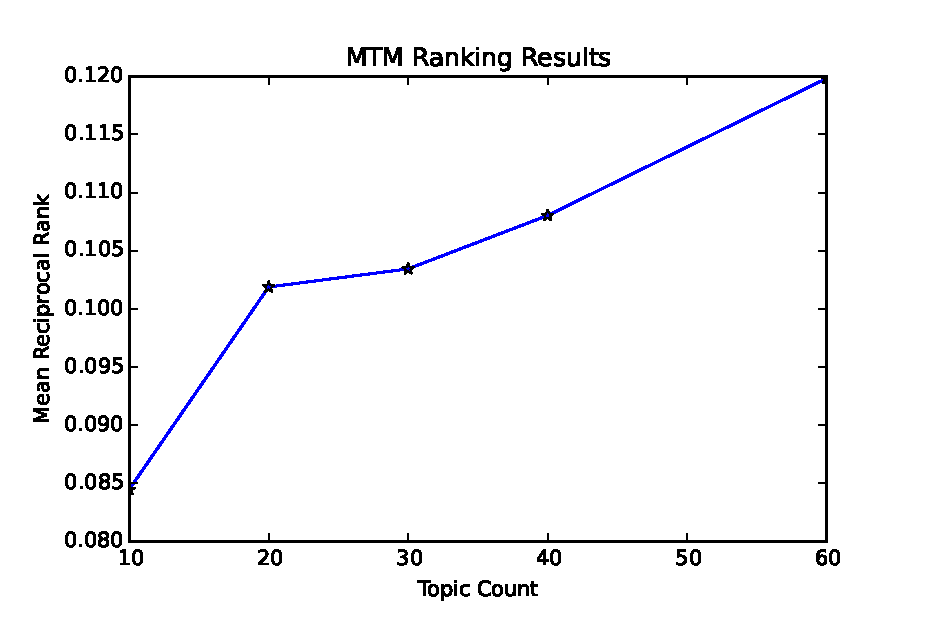
\includegraphics[width=0.5\textwidth]{/Users/bryanfeeney/Workspace/ArduCeime/Incidental/mrr.eps}
%  \caption{Mean reciprocal-rank results for our current model. The ideal score is 0.6164. \emph{I'm still running experiments up to 100 topics}}\label{fig:mrr}
%\end{figure}

The results for precision and recall at M are given in tables \ref{tbl:rtm}, \ref{tbl:mtm-old} and \ref{tbl:mtm-new}. The documents are grouped into subsets based on how many out-links they have. This is the ``group" column with the number of documents in each group in the ``count" column.

The mean reciprocal-rank for 25 topics for RTM, MTM-Old and MTM-New is are 0.0016, 0.0887 and 0.1050 respectively.

The perplexity for 25 topics for RTM, MTM-Old and MTM-New as evaluated on the \emph{training} dataset is 1581, 1559 and 1568 respectively. I just use this as a convergence check. The old MTM model does a better job of modelling words and links despite doing worse at ranking, but in reality it's simply focusing on words which outnumber links 300 to 1.

\begin{table}{\small
Precision at m\\
\begin{tabular}{| l | r || c | c | c | c | c | c | c | c | c |}\hline
 Group    & Count &    10 &    20 &    30 &    40 &    50 &    75 &   100 &   250 &   500  \\
\hline
  0,    3 &      2460 & 0.000 & 0.000 & 0.000 & 0.000 & 0.000 & 0.000 & 0.000 & 0.001 & 0.000  \\
  3,    5 &       634 & 0.000 & 0.000 & 0.001 & 0.001 & 0.001 & 0.001 & 0.001 & 0.001 & 0.001  \\
  5,   10 &       546 & 0.000 & 0.000 & 0.000 & 0.001 & 0.001 & 0.001 & 0.001 & 0.002 & 0.002  \\
 $\geq 10$ &        86 & 0.001 & 0.001 & 0.001 & 0.002 & 0.002 & 0.002 & 0.002 & 0.003 & 0.003  \\
\hline\end{tabular}\\

Recall at m\\
\begin{tabular}{| l | r || c | c | c | c | c | c | c | c | c |}\hline
 Group    & Count &    10 &    20 &    30 &    40 &    50 &    75 &   100 &   250 &   500  \\ \hline
  0,    3 &      2460 & 0.001 & 0.003 & 0.006 & 0.010 & 0.010 & 0.014 & 0.017 & 0.078 & 0.124  \\
  3,    5 &       634 & 0.000 & 0.002 & 0.004 & 0.009 & 0.010 & 0.013 & 0.016 & 0.060 & 0.102  \\
  5,   10 &       546 & 0.000 & 0.001 & 0.002 & 0.006 & 0.006 & 0.011 & 0.013 & 0.052 & 0.111  \\
 $\geq 10$ &        86 & 0.001 & 0.001 & 0.002 & 0.007 & 0.008 & 0.010 & 0.013 & 0.051 & 0.112  \\
\hline\end{tabular}
\caption{Precision and recall at m for the RTM model with 25 topics. Mean reciprocal rank is 0.0016}\label{tbl:rtm}
}\end{table}

\begin{table}{\small
Precision at m\\
\begin{tabular}{| l | r || c | c | c | c | c | c | c | c | c |}\hline
 Group    & Count &    10 &    20 &    30 &    40 &    50 &    75 &   100 &   250 &   500  \\
\hline
  0,    3 &      2460 & 0.032 & 0.022 & 0.017 & 0.015 & 0.013 & 0.010 & 0.009 & 0.005 & 0.003  \\
  3,    5 &       634 & 0.081 & 0.053 & 0.042 & 0.036 & 0.032 & 0.025 & 0.021 & 0.012 & 0.007  \\
  5,   10 &       546 & 0.121 & 0.080 & 0.065 & 0.056 & 0.049 & 0.039 & 0.033 & 0.020 & 0.012  \\
 $\geq 10$ &        86 & 0.208 & 0.142 & 0.112 & 0.096 & 0.083 & 0.066 & 0.056 & 0.033 & 0.021  \\
\hline\end{tabular}\\

Recall at m\\
\begin{tabular}{| l | r || c | c | c | c | c | c | c | c | c |}\hline
 Group    & Count &    10 &    20 &    30 &    40 &    50 &    75 &   100 &   250 &   500  \\ \hline
  0,    3 &      2460 & 0.180 & 0.239 & 0.288 & 0.332 & 0.365 & 0.434 & 0.491 & 0.695 & 0.832  \\
  3,    5 &       634 & 0.181 & 0.237 & 0.283 & 0.324 & 0.356 & 0.421 & 0.479 & 0.673 & 0.829  \\
  5,   10 &       546 & 0.168 & 0.221 & 0.269 & 0.311 & 0.338 & 0.403 & 0.457 & 0.675 & 0.823  \\
 $\geq 10$ &        86 & 0.165 & 0.225 & 0.264 & 0.300 & 0.325 & 0.388 & 0.441 & 0.646 & 0.815  \\
\hline\end{tabular}
\caption{Precision and recall at m for the old MTM model with 25 topics. Mean reciprocal rank is 0.0887}\label{tbl:mtm-old}
}\end{table}

\begin{table}{\small
Precision at m\\
\begin{tabular}{| l | r || c | c | c | c | c | c | c | c | c |}\hline
 Group    & Count &    10 &    20 &    30 &    40 &    50 &    75 &   100 &   250 &   500  \\
\hline
  0,    3 &      2460 & 0.045 & 0.031 & 0.024 & 0.020 & 0.017 & 0.013 & 0.010 & 0.005 & 0.003  \\
  3,    5 &       634 & 0.113 & 0.079 & 0.061 & 0.050 & 0.043 & 0.032 & 0.026 & 0.012 & 0.007  \\
  5,   10 &       546 & 0.155 & 0.113 & 0.092 & 0.077 & 0.066 & 0.051 & 0.041 & 0.020 & 0.012  \\
 $\geq 10$ &        86 & 0.245 & 0.179 & 0.147 & 0.124 & 0.108 & 0.083 & 0.068 & 0.033 & 0.019  \\
\hline\end{tabular}\\

Recall at m\\
\begin{tabular}{| l | r || c | c | c | c | c | c | c | c | c |}\hline
 Group    & Count &    10 &    20 &    30 &    40 &    50 &    75 &   100 &   250 &   500  \\ \hline
  0,    3 &      2460 & 0.253 & 0.348 & 0.403 & 0.441 & 0.476 & 0.535 & 0.571 & 0.680 & 0.772  \\
  3,    5 &       634 & 0.258 & 0.356 & 0.412 & 0.448 & 0.481 & 0.534 & 0.576 & 0.689 & 0.791  \\
  5,   10 &       546 & 0.215 & 0.316 & 0.381 & 0.425 & 0.458 & 0.526 & 0.567 & 0.692 & 0.795  \\
 $\geq 10$ &        86 & 0.193 & 0.283 & 0.348 & 0.394 & 0.427 & 0.492 & 0.535 & 0.659 & 0.766  \\
\hline\end{tabular}
\caption{Precision and recall at m for the current MTM model with 25 topics. Mean reciprocal rank is 0.1050}\label{tbl:mtm-new}
}\end{table}


\subsubsection*{Model Variants}
I looked into initialising the $\vv{\mu}$, $\Sigma$, $\Theta$ and $\vv{\beta}_1, \ldots, \vv{\beta}_k$ with the output of a CTM run, and then drawing $\Phi \sim \mnor{\Theta}{\diag{\vv{\rho}}}{\Sigma}$ however while that improved perplexity it caused the precision and recall scores to degrade.

I also looked at the effect of $\alpha$ and $\vv{\rho}$. Fixing these at 1 led to poorer perplexity, precision and recall metrics. The more interesting effect however that convergence was substantially slower (taking almost twice as many iterations) with $\rho_d$ fixed at 1. There may be benefit to taking into account variance at the document level during training, however I need to diagnose the issues with covariance to be sure. %With $\rho_d$ and $\alpha$ allowed vary, the new MTM model converged in half the number of iterations as the MTM-Old model. I haven't yet checked if this could work as a simple way of expediting inference in a vanilla correlated topic-model (CTM).

\section{Discussion}
In this model, I've re-used the same topic-covariance $\Sigma$ across both distributions. In practice, it's necessary to share a single covariance matrix in order to be able to obtain marginal distributions, in this case $\Phi \sim \mnor{0}{\alpha I_D + \diag{\vv{\rho}}}{\Sigma}$. I'm not sure that's sufficient justification for sharing the parameter. It is scaled in different ways by $\alpha$ and $\rho_d$ in both distributions, with $\rho_d$ always being greater than $\alpha$.

This model still doesn't take into account any temporal effects, i.e. that certain papers become less popular over time. 

I haven't made use of the authorship or venue features in this. I tried employing these in a separate model which derived topics for $\thd$ for document $d$ from features $\xd$ according to $\thd \sim \nor{A \xd}{\Sigma}$, and found that they gave no benefit, presumably the 3,000 words in each document provide sufficient information, such that authorship, venue and year are of no benefit. 

However there may be some benefit to features in terms of certain patterns observed in other research\cite{Bethard2010}, e.g. that authors self-cite, that they cite authors who cite them in turn, and that newer papers are more likely to be cited than old. \bibliographystyle{plain}
\bibliography{/Users/bryanfeeney/Documents/library.bib}

\end{document}
